\documentclass[11pt,fleqn,twoside]{article}
\usepackage{makeidx}
\makeindex
\usepackage{palatino} %or {times} etc
\usepackage{plain} %bibliography style 
\usepackage{amsmath} %math fonts - just in case
\usepackage{amsfonts} %math fonts
\usepackage{amssymb} %math fonts
\usepackage{lastpage} %for footer page numbers
\usepackage{fancyhdr} %header and footer package
\usepackage{mmpv2} 
\usepackage{url}

\usepackage{graphicx}
\usepackage{algpseudocode}

% the following packages are used for citations - You only need to include one. 
%
% Use the cite package if you are using the numeric style (e.g. IEEEannot). 
% Use the natbib package if you are using the author-date style (e.g. authordate2annot). 
% Only use one of these and comment out the other one. 
\usepackage{cite}
%\usepackage{natbib}

\begin{document}

\name{Alexander D. Brown}
\userid{adb9}
\projecttitle{Kyffin Williams: Digital Analysis of Paintings}
\projecttitlememoir{Kyffin Williams: Digital Analysis of Paintings} %same as the project title or abridged version for page header
\reporttitle{Progress Report}
\version{0.1}
\docstatus{Draft}
\modulecode{CS39440}
\supervisor{Hannah M. Dee} % e.g. Neil Taylor
\supervisorid{hmd1}
\wordcount{?} %TODO

%optional - comment out next line to use current date for the document
%\documentdate{26th October 2011} 
\mmp

\setcounter{tocdepth}{3} %set required number of level in table of contents
\tableofcontents
\listoffigures
\listoftables

\newpage

%==============================================================================
\section{Project Summary}
%==============================================================================
Sir John ``Kyffin'' Williams was a landscape painter from Wales whose work was predominantly based 
in Wales and Patagonia. His work, with associated metadata collected by Gareth Lloyd Roderick and 
the National Library of Wales, allows for some interesting analysis; particularly that of temporal 
or geological data for a given painting.

Temporal analysis will be the focus of this project as it allows for a diverse range of techniques;
from statistical analysis of RGB values of the paintings to looking at the length and style of 
paintbrush strokes. 

Whilst it would be nice to be able to predict the age of a painting with no known year, it is far
more interesting to try to guess the year of paintings where the date is known. This allows for
cross-validation of the techniques employed to guess the year. This project will use leave-one-out
cross-validation for simplicity as the data set is small enough to allow this computationally 
expensive technique.

%==============================================================================
\section{Current Progress}
%==============================================================================

\subsection{Design}
An initial UML class diagram is depicted by figure~\ref{fig:init-class}. This design will allow 
additional techniques, both analysis and machine learning based, to be added easily. Command line
arguments, or later a GUI front-end, will be used to specify which techniques should be used.

The GUI elements depicted are used for visualising the analysed data or results of the machine
learning algorithms.

\begin{figure}[p]
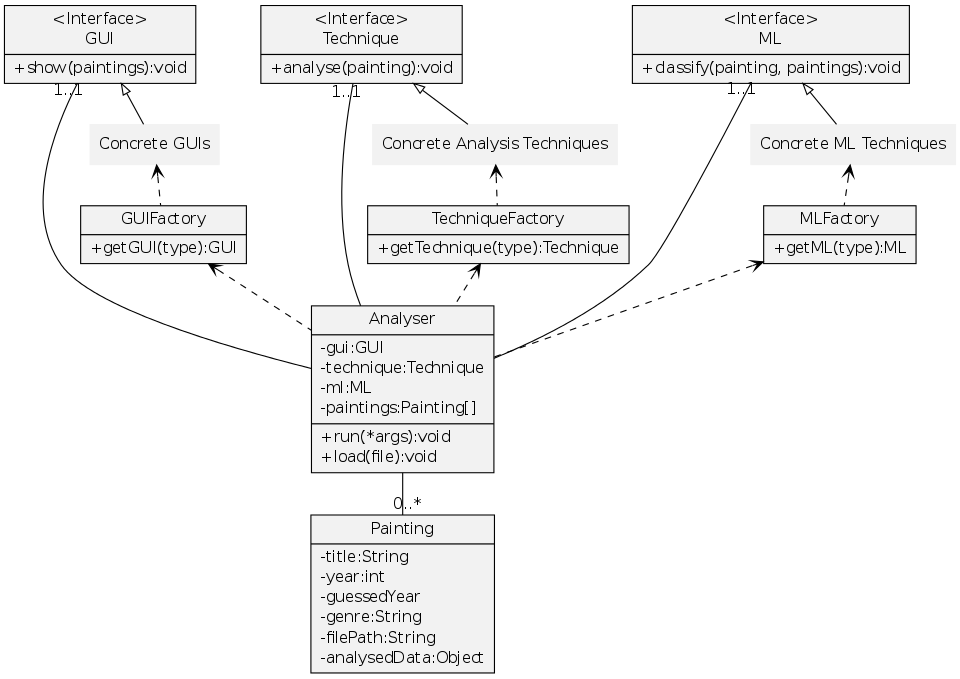
\includegraphics[scale=0.5]{img/design.png}
\caption{Initial Design}
\label{fig:init-class}
\end{figure}

\subsection{Colour Space Statistical Analysis}
With the design solidified, I begun to work on the statistical analysis of digital images. The 
easiest of these techniques is to read the image pixel by pixel, taking the various intensities at
that pixel, then averaging them out over the whole image.

The most common colour space used is RGB (Red, Green, Blue), where each pixel holds three different
intensities, one for each colour with a value of 0 to 255.

Using this analysis I plotted a graph of all paintings with a known year against the different 
intensities (see figure~\ref{fig:mean-rgb-by-year}). As can be seen from this graph, the RGB values
tend to fluctuate without much correlation between year.

\begin{figure}[p]
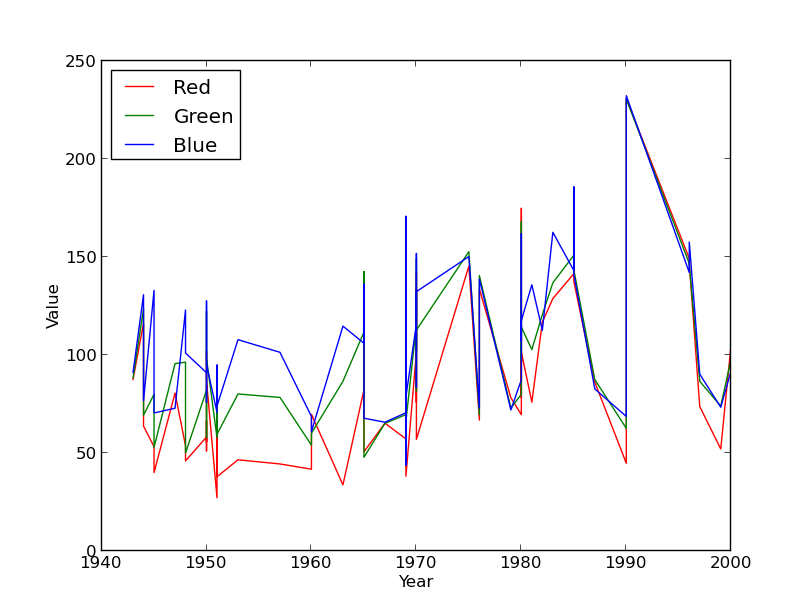
\includegraphics[scale=0.5]{img/kyffin-rgp-avg.png}
\caption{Mean RGB intensities by year.}
\label{fig:mean-rgb-by-year}
\end{figure}

Another popular colour space used in image processing is HSV (Hue, Saturation, Value) as it shows
variations in colour, saturation and brightness separately (unlike RGB where all three values are
affected by changes in brightness). It was a simple matter of changing the existing code for RGB
so that it would analyse HSV values instead.

I also decided it would be an improvement to average all values in the same year together to help
show changes as time goes on (see figure~\ref{fig:mean-hsv-by-year}).

\begin{figure}[p]
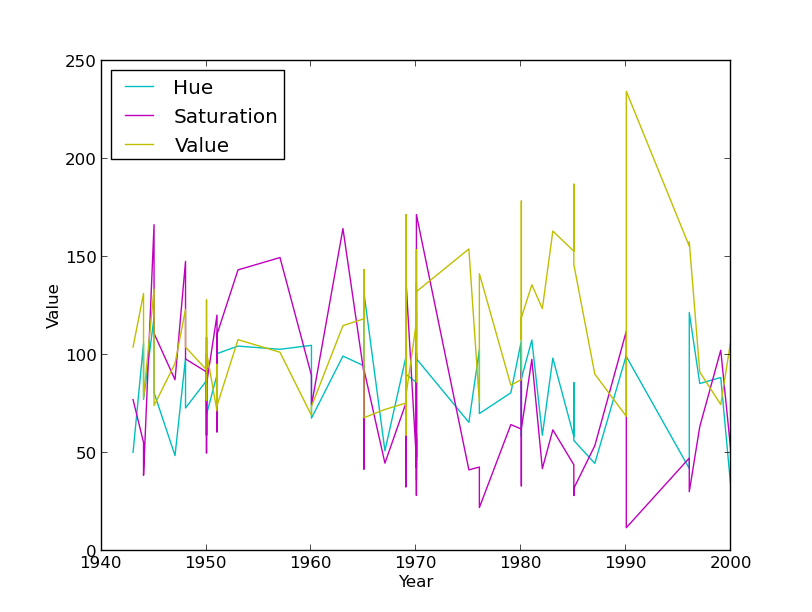
\includegraphics[scale=0.5]{img/hsv-legend-12-11-01.png}
\caption{Mean HSV intensities by year.}
\label{fig:mean-hsv-by-year}
\end{figure}


\subsection{Histogram Analysis}
With colour-space analysis complete, the next sensible step was to start generating colour 
histograms from Kyffin Williams paintings.

A histogram is a nice way of displaying the distribution of colour in a given image and is 
therefore a more useful representation of a painting than colour-space averages.

As with before, histograms can be taken from different colour spaces, currently only the program
can only generate RGB histograms, but it is trivial to include HSV histograms too.

\subsection{Nearest Neighbour Classification}
Having finished the analysis techniques, then next part was to create a simple classification 
algorithm. The simplest of which is 1-Nearest Neighbour, that is; take the ``Nearest'' training
example to the example to be classified and classify the year of this example with the year of the
nearest example (see figure~\ref{fig:1-nn}).

This simple algorithm can be expanded to be a K-Nearest Neighbour algorithm without too much effort
(see figure~\ref{fig:k-nn}).


\subsubsection{Distance Measures}
Working out the ``Nearest'' example(s) to a given painting requires some way of measuring distance
between the two.

One very simple way of doing this is Manhattan distance (figure~\ref{eq:manhattan}). This distance
measure can be improved further to euclidean distance (figure~\ref{eq:euclidea}) without too much
effort.

\begin{figure}[p]
\[
d = \sum^X_{x=0}{|a_x - b_x|}
\]

\(X\): All dimensions present in both \(a\) and \(b\).\\
\(a\): The first point.\\
\(b\): The second point.

\caption{Manhattan Distance}
\label{eq:manhattan}
\end{figure}

\begin{figure}[p]
\[
d = \sqrt{\sum^X_{x=0}{(a_x - b_x)^2}}
\]

\(X\): All dimensions present in both \(a\) and \(b\).\\
\(a\): The first point.\\
\(b\): The second point.
\caption{Euclidean Distance}
\label{eq:euclidean}
\end{figure}

\begin{figure}
\begin{algorithmic}
\State $bestDistance \gets \infty$
\For{$x = 1 \to X$}
	\If{$distance(a, x) < bestDistance$}
		\State $bestDistance \gets distance(a, x)$
	\EndIf
\EndFor
\end{algorithmic}

Where:\\
\(a\) is the example to classify.\\
\(X\) is the list of all training examples.
\caption{1-Nearest Neighbour}
\label{fig:1-nn}
\end{figure}

\begin{figure}
\begin{algorithmic}
\State $kBest \gets []$
\For{$x = 1 \to X$}
	\State $cur \gets distance(a, x)$
	\For{$k = 1 \to K$}
		\If{$cur < kBest[k]$}
			\State $temp \gets kBest[k]$
			\State $kBest[k] \gets cur$
			\State $cur \gets temp$
		\EndIf
	\EndFor
\EndFor
\end{algorithmic}
Where:\\
$a$ is the example to classify.\\
$X$ is the list of all training examples.
$K$ is the number of nearest neighbours to check.
\caption{K-Nearest Neighbour}
\label{fig:k-nn}
\end{figure}

%==============================================================================
\section{Planning}
%==============================================================================

%
% Start to comment out / remove the following lines. They are only provided for instruction for this example template.  You don't need the following section title, because it will be added as part of the bibliography section. 
%
%==============================================================================
\section*{Your Bibliography - REMOVE for final version}
%==============================================================================
%
You need to include an annotated bibliography. This should list all relevant web pages, books, journals etc. that you have consulted in researching your project. Each reference should include an annotation. 

The purpose of the section is to understand what sources you are looking at.  A correctly formatted list of items is sufficient. You might go further and make use of bibliographic tools, e.g. BibTeX in a LaTeX document, could be used to provide citations, for example \cite{NumericalRecipes} \cite{MarksPaper} \cite[99-101]{FailBlog} \cite{kittenpic_ref}.  The bibliographic tools are not a requirement, but you are welcome to use them.   

You can remove the above {\em Your Bibliography} section heading because it will be added in by the renewcommand which is part of the bibliography. The correct annotated bibliography information is provided below. 
%
% End of comment out / remove the lines. They are only provided for instruction for this example template. 
%


\nocite{*} % include everything from the bibliography, irrespective of whether it has been referenced.

% the following line is included so that the bibliography is also shown in the table of contents. There is the possibility that this is added to the previous page for the bibliography. To address this, a newline is added so that it appears on the first page for the bibliography. 
\newpage
\addcontentsline{toc}{section}{Annotated Bibliography} 

%
% example of including an annotated bibliography. The current style is an author date one. If you want to change, comment out the line and uncomment the subsequent line. You should also modify the packages included at the top (see the notes earlier in the file) and then trash your aux files and re-run. 
%\bibliographystyle{authordate2annot}
\bibliographystyle{IEEEannot}
\renewcommand{\refname}{Annotated Bibliography}  % if you put text into the final {} on this line, you will get an extra title, e.g. References. This isn't necessary for the outline project specification. 
\bibliography{mmp} % References file


\end{document}
